\documentclass{beamer}


% Theme and page layout
\usetheme{gapz}
\setbeamertemplate{navigation symbols}{}

% Fonts
\usepackage{fontspec}
\defaultfontfeatures{Mapping=tex-text,Scale=MatchLowercase,Numbers=Lining}
%\setsansfont[
%	ItalicFont = Whitney MediumItalic,
%	BoldFont = Whitney Semibold,
%	BoldItalicFont = Whitney SemiboldItalic,
%	SmallCapsFont = Whitney MediumSC
%]{Whitney Medium}

% Language
\usepackage{polyglossia}
\setdefaultlanguage{english}

% Graphics
\usepackage{graphicx}
\graphicspath{{./images/}}



\title{Three-dimensional modeling and printing project}
\subtitle{}
\author[V. D., A. L., C. N., J. P., F. R.]{\begin{scriptsize}
Vincent~Duvert \\ Antoine~Lubineau \\ Caroline~Naud \\ James~Packer \\ Florian~Ribon\end{scriptsize}}
\date{from January 23 to March 16, 2012}

\titlegraphic{
\includegraphics[width=4cm]{inp-enseeiht}}

\begin{document}

\frame{\titlepage}

\section{Presentation of the project}

\subsection{The client team}
\begin{frame}
	\frametitle{The client team}
	
	\begin{block}{The \textsc{VORTEX} team}
    \end{block}
    
    \begin{center}
		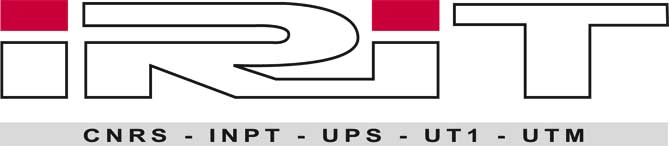
\includegraphics[width=4cm]{irit}	
	\end{center}
    
\end{frame}

\subsection{The resources}
\begin{frame}
	\frametitle{The resources}
	
	\begin{block}{The project team}
    \end{block}
    
    \begin{block}{The material resources}
    \end{block}
      
\end{frame}

\begin{frame}
	\frametitle{Ultimaker 3D printer}

    \begin{center}
		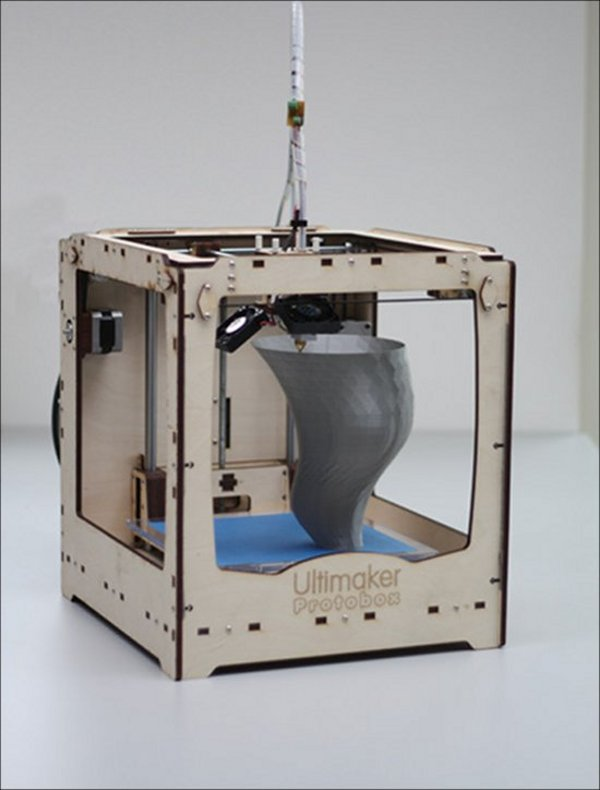
\includegraphics[width=4cm]{Ultimaker}	
	\end{center}
    
\end{frame}

\subsection{The objectives}
\begin{frame}
	\frametitle{blablabla}
    
\end{frame}

\section{About the project management ...}
\begin{frame}
	\frametitle{The V cycle management strategy}

    \begin{center}
		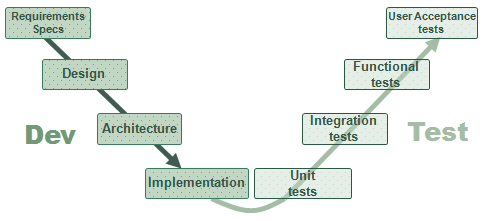
\includegraphics[width=8cm]{VCycle}	
	\end{center}
\end{frame}

\section{Architecture of the project}
\begin{frame}
	\frametitle{blabla}

    \begin{center}
		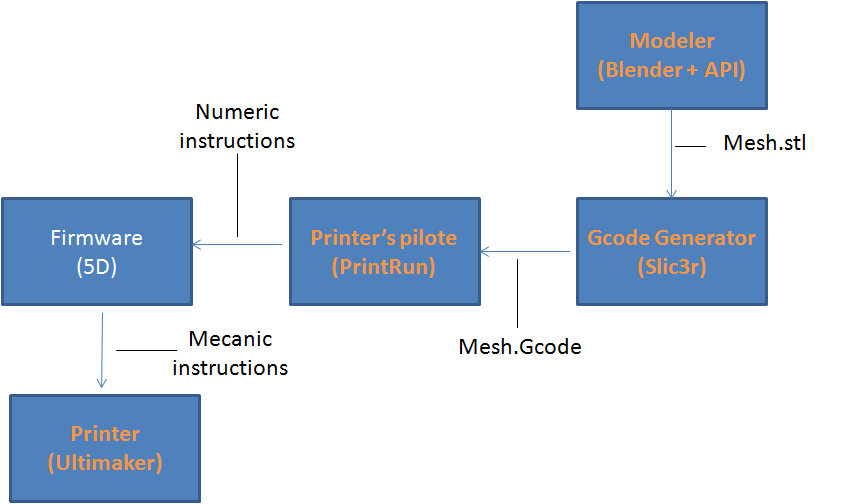
\includegraphics[width=8cm]{ARD1}	
	\end{center}
	
\end{frame}

\section{Mesh correction}
\begin{frame}
	\frametitle{blabla}

    \begin{block}{blabla}
    \end{block}
\end{frame}

\section{Modifications in Blender's interface}
\begin{frame}
	\frametitle{blabla}

    \begin{block}{blabla}
    \end{block}
\end{frame}

\section{Calibration of the printer}
\begin{frame}
	\frametitle{blabla}

    \begin{block}{blabla}
    \end{block}
\end{frame}

\section{Conclusions and thanks}
\begin{frame}
	\frametitle{blabla}

    \begin{block}{blablabla}
    \end{block}
\end{frame}

\begin{frame}
	\frametitle{}

    \begin{center}
    \Large{Thank you for your attention !}
    \end{center}
\end{frame}
	
\end{document}
